\numoptstrue
\yearpaper{2021}{12 September 2021 \textperiodcentered{} Test Booklet Code M4 \textperiodcentered{} Physics Q 1--50 (Section A: 1--35, Section B: 36--50, any 10 of 15) \textperiodcentered{} 180 Marks}{}
\begin{multicols}{2}

\QQ{Consider the following statements (A) and (B) and identify the correct answer.
\begin{stmts}[(\Alph*)]
\item A zener diode is connected in reverse bias, when used as a voltage regulator.
\item The potential barrier of p-n junction lies between 0.1\,V to 0.3\,V.
\end{stmts}}
{\opt{(A) and (B) both are correct.}{(A) and (B) both are incorrect.}{(A) is correct and (B) is incorrect.}{(A) is incorrect but (B) is correct.}}

\QQ{A capacitor of capacitance `$C$', is connected across an ac source of voltage $V$, given by $V = V_0\sin\omega t$. The displacement current between the plates of the capacitor, would then be given by:}
{\opt{$I_d = V_0\omega C\cos\omega t$}{$I_d = \dfrac{V_0}{\omega C}\cos\omega t$}{$I_d = \dfrac{V_0}{\omega C}\sin\omega t$}{$I_d = V_0\omega C\sin\omega t$}}

\QQ{A body is executing simple harmonic motion with frequency `$n$', the frequency of its potential energy is:}
{\opt{$n$}{$2n$}{$3n$}{$4n$}}

\QQ{The equivalent capacitance of the combination shown in the figure is:
\fig{\begin{circuitikz}[scale=0.62,transform shape,font=\Large]
\draw (-0.8,1) -- (0,1) -- (0,2) to[C,l=$C$] (2,2) -- (4,2) -- (4,1) -- (4.8,1);
\draw (0,1) -- (0,0) to[C,l_=$C$] (2,0) -- (4,0) -- (4,1);
\draw (2,2) to[C,l=$C$] (2,0);
\end{circuitikz}}}
{\opt{$3C$}{$2C$}{$C/2$}{$3C/2$}}

\QQ{Find the value of the angle of emergence from the prism. Refractive index of the glass is $\sqrt3$.
\fig{\begin{tikzpicture}[scale=0.8]
\draw (0,0) -- (2,0) -- (0,2) -- cycle; \draw (0,0) rectangle (0.15,0.15);
\draw (1.6,0) arc (180:135:0.4); \node[lbl] at (1.45,0.2) {$60^\circ$};
\draw[->] (1.6,1.6) -- (1.0,1.0); \draw (1.0,1.0) ++(0.12,0.12) -- ++(0.12,-0.12) -- ++(-0.12,-0.12);
\end{tikzpicture}}}
{\opt{$60^\circ$}{$30^\circ$}{$45^\circ$}{$90^\circ$}}

\QQ{A dipole is placed in an electric field as shown. In which direction will it move?
\fig{\begin{tikzpicture}[scale=0.8]
\draw[densely dashed,->] (0,0) -- (2.6,0) node[right,lbl]{$\vec E$}; \draw[densely dashed,->] (0,0) -- (2.2,1.2); \draw[densely dashed,->] (0,0) -- (2.2,-1.2);
\fill (1.0,0.15) circle (1.5pt) node[below,lbl]{$+q$}; \fill (1.6,0.15) circle (1.5pt) node[below,lbl]{$-q$}; \draw (1.0,0.15) -- (1.6,0.15);
\end{tikzpicture}}}
{\opt{towards the left as its potential energy will increase.}{towards the right as its potential energy will decrease.}{towards the left as its potential energy will decrease.}{towards the right as its potential energy will increase.}}

\QQ{Match Column-I and Column-II and choose the correct match from the given choices.\par\smallskip
\begin{tabular}{@{}lp{0.42\linewidth}ll@{}}
\multicolumn{2}{@{}l}{\textit{Column-I}} & \multicolumn{2}{l}{\textit{Column-II}}\\
(A) & Root mean square speed of gas molecules & (P) & $\frac13nm\bar v^2$\\
(B) & Pressure exerted by ideal gas & (Q) & $\sqrt{\frac{3RT}M}$\\
(C) & Average kinetic energy of a molecule & (R) & $\frac52RT$\\
(D) & Total internal energy of 1 mole of a diatomic gas & (S) & $\frac32k_BT$
\end{tabular}}
{\opt{(A)-(R), (B)-(P), (C)-(S), (D)-(Q)}{(A)-(Q), (B)-(R), (C)-(S), (D)-(P)}{(A)-(Q), (B)-(P), (C)-(S), (D)-(R)}{(A)-(R), (B)-(Q), (C)-(P), (D)-(S)}}

\QQ{A convex lens `A' of focal length $20\unit{cm}$ and a concave lens `B' of focal length $5\unit{cm}$ are kept along the same axis with a distance `$d$' between them. If a parallel beam of light falling on `A' leaves `B' as a parallel beam, then the distance `$d$' in cm will be:}
{\opt{25}{15}{50}{30}}

\QQ{If force [F], acceleration [A] and time [T] are chosen as the fundamental physical quantities. Find the dimensions of energy.}
{\opt{[F][A][T]}{[F][A][T$^2$]}{[F][A][T$^{-1}$]}{[F][A$^{-1}$][T]}}

\QQ{A cup of coffee cools from $90^\circ$C to $80^\circ$C in $t$ minutes, when the room temperature is $20^\circ$C. The time taken by a similar cup of coffee to cool from $80^\circ$C to $60^\circ$C at a room temperature same at $20^\circ$C is:}
{\opt{$\dfrac{13}{10}t$}{$\dfrac{13}5t$}{$\dfrac{10}{13}t$}{$\dfrac5{13}t$}}

\QQ{A particle is released from height $S$ from the surface of the Earth. At a certain height its kinetic energy is three times its potential energy. The height from the surface of earth and the speed of the particle at that instant are respectively:}
{\opt{$\dfrac S4,\ \dfrac{3gS}2$}{$\dfrac S4,\ \dfrac{\sqrt{3gS}}2$}{$\dfrac S2,\ \dfrac{\sqrt{3gS}}2$}{$\dfrac S4,\ \sqrt{\dfrac{3gS}2}$}}

\QQ{The velocity of a small ball of mass $M$ and density $d$, when dropped in a container filled with glycerine becomes constant after some time. If the density of glycerine is $\dfrac d2$, then the viscous force acting on the ball will be:}
{\opt{$\dfrac{Mg}2$}{$Mg$}{$\dfrac32Mg$}{$2Mg$}}

\QQ{For a plane electromagnetic wave propagating in $x$-direction, which one of the following combination gives the correct possible directions for electric field ($E$) and magnetic field ($B$) respectively?}
{\opt{$\hat j+\hat k$, $\hat j+\hat k$}{$-\hat j+\hat k$, $-\hat j-\hat k$}{$\hat j+\hat k$, $-\hat j-\hat k$}{$-\hat j+\hat k$, $-\hat j+\hat k$}}

\QQ{Column-I gives certain physical terms associated with flow of current through a metallic conductor. Column-II gives some mathematical relations involving electrical quantities. Match Column-I and Column-II with appropriate relations.\par\smallskip
\begin{tabular}{@{}ll@{\quad}ll@{}}
(A) & Drift Velocity & (P) & $\dfrac m{ne^2\rho}$\\[4pt]
(B) & Electrical Resistivity & (Q) & $nev_d$\\[2pt]
(C) & Relaxation Period & (R) & $\dfrac{eE}m\tau$\\[4pt]
(D) & Current Density & (S) & $\dfrac EJ$
\end{tabular}}
{\opt{(A)-(R), (B)-(S), (C)-(P), (D)-(Q)}{(A)-(R), (B)-(S), (C)-(Q), (D)-(P)}{(A)-(R), (B)-(P), (C)-(S), (D)-(Q)}{(A)-(R), (B)-(Q), (C)-(S), (D)-(P)}}

\QQ{A spring is stretched by $5\unit{cm}$ by a force $10\unit{N}$. The time period of the oscillations when a mass of $2\unit{kg}$ is suspended by it is:}
{\opt{0.0628\,s}{6.28\,s}{3.14\,s}{0.628\,s}}

\QQ{A parallel plate capacitor has a uniform electric field `$\vec E$' in the space between the plates. If the distance between the plates is `$d$' and the area of each plate is `$A$', the energy stored in the capacitor is: ($\varepsilon_0$ = permittivity of free space)}
{\opt{$\dfrac12\varepsilon_0E^2$}{$\varepsilon_0EAd$}{$\dfrac12\varepsilon_0E^2Ad$}{$\dfrac{E^2Ad}{\varepsilon_0}$}}

\QQ{An infinitely long straight conductor carries a current of $5\unit{A}$ as shown. An electron is moving with a speed of $10^5\unit{m/s}$ parallel to the conductor. The perpendicular distance between the electron and the conductor is $20\unit{cm}$ at an instant. Calculate the magnitude of the force experienced by the electron at that instant.
\fig{\begin{tikzpicture}[scale=0.8]
\draw[->] (0,0) node[left,lbl]{P} -- (2.6,0) node[right,lbl]{Q}; \node[lbl,below] at (1.6,0) {5\,A};
\draw (1,0) -- (1,1.4); \draw[->] (1,1.4) -- (2.2,1.4) node[above,lbl]{Electron $v = 10^5\unit{m/s}$};
\draw[<->] (1.3,0.05) -- (1.3,1.35) node[midway,right,lbl]{20\,cm};
\end{tikzpicture}}}
{\opt{$4\times10^{-20}\unit{N}$}{$8\pi\times10^{-20}\unit{N}$}{$4\pi\times10^{-20}\unit{N}$}{$8\times10^{-20}\unit{N}$}}

\QQ{A lens of large focal length and large aperture is best suited as an objective of an astronomical telescope since:}
{\opt{a large aperture contributes to the quality and visibility of the images.}{a large area of the objective ensures better light gathering power.}{a large aperture provides a better resolution.}{all of the above.}}

\QQ{A radioactive nucleus ${}^A_Z$X undergoes spontaneous decay in the sequence ${}^A_Z\mathrm X\to{}_{Z-1}\mathrm B\to{}_{Z-3}\mathrm C\to{}_{Z-2}\mathrm D$, where $Z$ is the atomic number of element X. The possible decay particles in the sequence are:}
{\opt{$\alpha$, $\beta^-$, $\beta^+$}{$\alpha$, $\beta^+$, $\beta^-$}{$\beta^+$, $\alpha$, $\beta^-$}{$\beta^-$, $\alpha$, $\beta^+$}}

\QQ{An inductor of inductance $L$, a capacitor of capacitance $C$ and a resistor of resistance `$R$' are connected in series to an ac source of potential difference `$V$' volts as shown in figure. Potential difference across L, C and R is $40\unit{V}$, $10\unit{V}$ and $40\unit{V}$, respectively. The amplitude of current flowing through LCR series circuit is $10\sqrt2\unit{A}$. The impedance of the circuit is:
\fig{\begin{circuitikz}[scale=0.62,transform shape,font=\Large]
\draw (0,2) to[L] (2,2) to[C] (3.5,2) to[R] (5.5,2) -- (5.5,0) -- (3.5,0) to[sV,l_=$V$] (2,0) -- (0,0) -- (0,2);
\node at (1,1.2) {40\,V}; \node at (2.75,1.2) {10\,V}; \node at (4.5,1.2) {40\,V};
\end{circuitikz}}}
{\opt{$4\sqrt2\unit{\Omega}$}{$5/\sqrt2\unit{\Omega}$}{$4\unit{\Omega}$}{$5\unit{\Omega}$}}

\QQ{The escape velocity from the Earth's surface is $v$. The escape velocity from the surface of another planet having a radius, four times that of Earth and same mass density is:}
{\opt{$v$}{$2v$}{$3v$}{$4v$}}

\QQ{A screw gauge gives the following readings when used to measure the diameter of a wire: Main scale reading: 0\,mm; Circular scale reading: 52 divisions. Given that 1\,mm on main scale corresponds to 100 divisions on the circular scale. The diameter of the wire from the above data is:}
{\opt{0.52\,cm}{0.026\,cm}{0.26\,cm}{0.052\,cm}}

\QQ{Water falls from a height of $60\unit{m}$ at the rate of $15\unit{kg/s}$ to operate a turbine. The losses due to frictional force are 10\% of the input energy. How much power is generated by the turbine? ($g = 10\unit{m/s^2}$)}
{\opt{10.2\,kW}{8.1\,kW}{12.3\,kW}{7.0\,kW}}

\QQ{A small block slides down on a smooth inclined plane, starting from rest at time $t = 0$. Let $S_n$ be the distance travelled by the block in the interval $t = n-1$ to $t = n$. Then, the ratio $\dfrac{S_n}{S_{n+1}}$ is:}
{\opt{$\dfrac{2n-1}{2n}$}{$\dfrac{2n-1}{2n+1}$}{$\dfrac{2n+1}{2n-1}$}{$\dfrac{2n}{2n-1}$}}

\QQ{Polar molecules are the molecules:}
{\opt{having zero dipole moment.}{acquire a dipole moment only in the presence of electric field due to displacement of charges.}{acquire a dipole moment only when magnetic field is absent.}{having a permanent electric dipole moment.}}

\QQ{A thick current carrying cable of radius `$R$' carries current `$I$' uniformly distributed across its cross-section. The variation of magnetic field $B(r)$ due to the cable with the distance `$r$' from the axis of the cable is represented by:}
{\optfig{\gaxes{$r$}{$B$}{\draw (0,0) .. controls (1.0,0.1) and (1.6,0.5) .. (1.8,1.7);}}
{\gaxes{$r$}{$B$}{\draw (0,0) -- (1.7,1.5);}}
{\gaxes{$r$}{$B$}{\draw (0,0) -- (0.6,1.3) .. controls (1.0,0.6) and (1.3,0.35) .. (1.9,0.3); \draw[densely dashed] (0.6,1.3) -- (0.6,0);}}
{\gaxes{$r$}{$B$}{\draw (0,0) .. controls (0.2,1.0) and (0.6,1.4) .. (1.8,1.45);}}}

\QQ{In a potentiometer circuit a cell of EMF 1.5\,V gives balance point at $36\unit{cm}$ length of wire. If another cell of EMF 2.5\,V replaces the first cell, then at what length of the wire, the balance point occurs?}
{\opt{60\,cm}{21.6\,cm}{64\,cm}{62\,cm}}

\QQ{Two charged spherical conductors of radius $R_1$ and $R_2$ are connected by a wire. Then the ratio of surface charge densities of the spheres ($\sigma_1/\sigma_2$) is:}
{\opt{$\dfrac{R_1}{R_2}$}{$\dfrac{R_2}{R_1}$}{$\sqrt{\dfrac{R_1}{R_2}}$}{$\dfrac{R_1^2}{R_2^2}$}}

\QQ{An electromagnetic wave of wavelength `$\lambda$' is incident on a photosensitive surface of negligible work function. If `$m$' mass is of photoelectron emitted from the surface has de-Broglie wavelength $\lambda_d$, then:}
{\opt{$\lambda = \left(\dfrac{2m}{hc}\right)\lambda_d^2$}{$\lambda_d = \left(\dfrac{2mc}h\right)\lambda^2$}{$\lambda = \left(\dfrac{2mc}h\right)\lambda_d^2$}{$\lambda = \left(\dfrac{2h}{mc}\right)\lambda_d^2$}}

\QQ{The electron concentration in an n-type semiconductor is the same as hole concentration in a p-type semiconductor. An external field (electric) is applied across each of them. Compare the currents in them.}
{\opt{current in n-type = current in p-type.}{current in p-type $>$ current in n-type.}{current in n-type $>$ current in p-type.}{No current will flow in p-type, current will only flow in n-type.}}

\QQ{The number of photons per second on an average emitted by the source of monochromatic light of wavelength $600\unit{nm}$, when it delivers the power of $3.3\times10^{-3}$ watt will be: ($h = 6.6\times10^{-34}\unit{J\,s}$)}
{\opt{$10^{18}$}{$10^{17}$}{$10^{16}$}{$10^{15}$}}

\QQ{If E and G respectively denote energy and gravitational constant, then $\dfrac EG$ has the dimensions of:}
{\opt{[M$^2$][L$^{-1}$][T$^0$]}{[M][L$^{-1}$][T$^{-1}$]}{[M][L$^0$][T$^0$]}{[M$^2$][L$^{-2}$][T$^{-1}$]}}

\QQ{The effective resistance of a parallel connection that consists of four wires of equal length, equal area of cross-section and same material is $0.25\unit{\Omega}$. What will be the effective resistance if they are connected in series?}
{\opt{0.25\,$\Omega$}{0.5\,$\Omega$}{1\,$\Omega$}{4\,$\Omega$}}

\QQ{The half-life of a radioactive nuclide is 100 hours. The fraction of original activity that will remain after 150 hours would be:}
{\opt{1/2}{$\dfrac1{2\sqrt2}$}{$\dfrac23$}{$\dfrac2{3\sqrt2}$}}

\QQ{A nucleus with mass number 240 breaks into two fragments each of mass number 120, the binding energy per nucleon of unfragmented nuclei is 7.6\,MeV while that of fragments is 8.5\,MeV. The total gain in the Binding Energy in the process is:}
{\opt{0.9\,MeV}{9.4\,MeV}{804\,MeV}{216\,MeV}}

\QQ{Two conducting circular loops of radii $R_1$ and $R_2$ are placed in the same plane with their centres coinciding. If $R_1\gg R_2$, the mutual inductance M between them will be directly proportional to:}
{\opt{$\dfrac{R_1}{R_2}$}{$\dfrac{R_2}{R_1}$}{$\dfrac{R_1^2}{R_2}$}{$\dfrac{R_2^2}{R_1}$}}

\QQ{In the product $\vec F = q(\vec v\times\vec B) = q\vec v\times(B\hat i+B\hat j+B_0\hat k)$. For $q = 1$ and $\vec v = 2\hat i+4\hat j+6\hat k$ and $\vec F = 4\hat i-20\hat j+12\hat k$. What will be the complete expression for $\vec B$?}
{\opt{$-8\hat i-8\hat j-6\hat k$}{$-6\hat i-6\hat j-8\hat k$}{$8\hat i+8\hat j-6\hat k$}{$6\hat i+6\hat j-8\hat k$}}

\QQ{For the given circuit, the input digital signals are applied at the terminals A, B and C. What would be the output at the terminal $y$?
\fig{\begin{tikzpicture}[xscale=0.6,yscale=0.5]
\foreach \x/\l in {1/t_1,2/t_2,3/t_3,4/t_4,5/t_5,6/t_6} {\draw[densely dashed] (\x,-4.6) -- (\x,0.5); \node[font=\tiny] at (\x,0.9) {$\l$};}
\node[lbl,left] at (-0.2,0) {A}; \draw (0,-0.6) -- (1,-0.6) -- (1,0) -- (2,0) -- (2,-0.6) -- (3,-0.6) -- (3,0) -- (4,0) -- (4,-0.6) -- (5,-0.6) -- (5,0) -- (6,0) -- (6,-0.6) -- (7,-0.6);
\node[lbl,left] at (-0.2,-2) {B}; \draw (0,-2.4) -- (2,-2.4) -- (2,-1.8) -- (4,-1.8) -- (4,-2.4) -- (7,-2.4);
\node[lbl,left] at (-0.2,-4) {C}; \draw (0,-3.6) -- (2,-3.6) -- (2,-4.2) -- (4,-4.2) -- (4,-3.6) -- (7,-3.6);
\end{tikzpicture}}
\fig{\begin{circuitikz}[scale=0.75,transform shape]
\draw (0,1) node[and port](G1){}; \draw (0,-1) node[nand port](G2){}; \draw (2.4,0) node[or port](G3){};
\draw (G1.in 1) -- ++(-0.8,0) node[ocirc]{} node[left]{A}; \draw (G2.in 2) -- ++(-0.8,0) node[ocirc]{} node[left]{C};
\draw (G1.in 2) -- ++(-0.4,0) |- (G2.in 1); \draw ($(G1.in 2)+(-0.4,-1)$) -- ++(-0.4,0) node[ocirc]{} node[left]{B};
\draw (G1.out) -| (G3.in 1); \draw (G2.out) -| (G3.in 2); \draw (G3.out) -- ++(0.4,0) node[ocirc]{} node[right]{$y$};
\end{circuitikz}}}
{\optfig{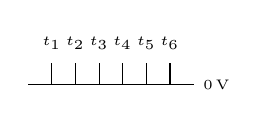
\begin{tikzpicture}[xscale=0.3,yscale=0.35]\foreach \x in {1,...,6} \node[font=\tiny] at (\x,1.5) {$t_\x$};\draw (0,0) -- (7,0) node[right,font=\tiny]{0\,V}; \foreach \x in {1,6} \draw (\x,0) -- (\x,0.8); \foreach \x in {2,...,5} \draw[thin] (\x,0) -- (\x,0.8);\end{tikzpicture}}{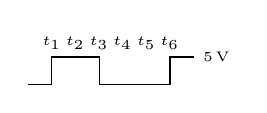
\begin{tikzpicture}[xscale=0.3,yscale=0.35]\foreach \x in {1,...,6} \node[font=\tiny] at (\x,1.5) {$t_\x$};\draw (0,0) -- (1,0) -- (1,1) -- (3,1) -- (3,0) -- (6,0) -- (6,1) -- (7,1) node[right,font=\tiny]{5\,V};\end{tikzpicture}}{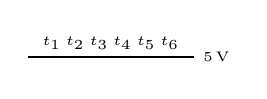
\begin{tikzpicture}[xscale=0.3,yscale=0.35]\foreach \x in {1,...,6} \node[font=\tiny] at (\x,1.5) {$t_\x$};\draw (0,1) -- (7,1) node[right,font=\tiny]{5\,V};\end{tikzpicture}}{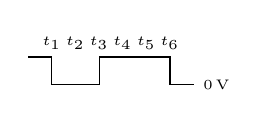
\begin{tikzpicture}[xscale=0.3,yscale=0.35]\foreach \x in {1,...,6} \node[font=\tiny] at (\x,1.5) {$t_\x$};\draw (0,1) -- (1,1) -- (1,0) -- (3,0) -- (3,1) -- (6,1) -- (6,0) -- (7,0) node[right,font=\tiny]{0\,V};\end{tikzpicture}}}

\QQ{A series LCR circuit containing $5.0\unit{H}$ inductor, $80\unit{\mu F}$ capacitor and $40\unit{\Omega}$ resistor is connected to $230\unit{V}$ variable frequency ac source. The angular frequencies of the source at which power transferred to the circuit is half the power at the resonant angular frequency are likely to be:}
{\opt{25\,rad/s and 75\,rad/s}{50\,rad/s and 25\,rad/s}{46\,rad/s and 54\,rad/s}{42\,rad/s and 58\,rad/s}}

\QQ{A uniform rod of length $200\unit{cm}$ and mass $500\unit{g}$ is balanced on a wedge placed at $40\unit{cm}$ mark. A mass of $2\unit{kg}$ is suspended from the rod at $20\unit{cm}$ and another unknown mass `$m$' is suspended from the rod at $160\unit{cm}$ mark as shown in the figure. Find the value of `$m$' such that the rod is in equilibrium. ($g = 10\unit{m/s^2}$)
\fig{\begin{tikzpicture}[scale=0.8]
\draw (0,0) rectangle (4,0.35); \node[lbl,above] at (0,0.35) {0}; \node[lbl,above] at (0.45,0.75) {20\,cm}; \node[lbl,above] at (0.9,0.35) {40\,cm}; \node[lbl,above] at (3.2,0.35) {160\,cm};
\draw (0.8,-0.15) -- (0.95,0) -- (0.65,0) -- cycle; \draw (0.4,0) -- (0.4,-0.6); \draw (0.05,-0.6) rectangle (0.75,-1.0) node[midway,lbl]{2\,kg};
\draw (3.2,0) -- (3.2,-0.6); \draw (2.95,-0.6) rectangle (3.45,-1.0) node[midway,lbl]{$m$};
\end{tikzpicture}}}
{\opt{$\dfrac12$\,kg}{$\dfrac13$\,kg}{$\dfrac16$\,kg}{$\dfrac1{12}$\,kg}}

\QQ{A point object is placed at a distance of $60\unit{cm}$ from a convex lens of focal length $30\unit{cm}$. If a plane mirror were put perpendicular to the principal axis of the lens and at a distance of $40\unit{cm}$ from it, the final image would be formed at a distance of:}
{\opt{20\,cm from the lens, it would be a real image.}{30\,cm from the lens, it would be a real image.}{30\,cm from the plane mirror, it would be a virtual image.}{20\,cm from the plane mirror, it would be a virtual image.}}

\QQ{A car starts from rest and accelerates at $5\unit{m/s^2}$. At $t = 4\unit{s}$, a ball is dropped out of a window by a person sitting in the car. What is the velocity and acceleration of the ball at $t = 6\unit{s}$? (Take $g = 10\unit{m/s^2}$)}
{\opt{20\,m/s, 5\,m/s$^2$}{20\,m/s, 0}{$20\sqrt2$\,m/s, 0}{$20\sqrt2$\,m/s, 10\,m/s$^2$}}

\QQ{Twenty seven drops of same size are charged at $220\unit{V}$ each. They combine to form a bigger drop. Calculate the potential of the bigger drop.}
{\opt{660\,V}{1320\,V}{1520\,V}{1980\,V}}

\QQ{A uniform conducting wire of length $12a$ and resistance `$R$' is wound up as a current carrying coil in the shape of, (i) an equilateral triangle of side `$a$', (ii) a square of side `$a$'. The magnetic dipole moments of the coil in each case respectively are:}
{\opt{$\sqrt3Ia^2$ and $3Ia^2$}{$3Ia^2$ and $Ia^2$}{$3Ia^2$ and $4Ia^2$}{$4Ia^2$ and $3Ia^2$}}

\QQ{A ball of mass $0.15\unit{kg}$ is dropped from a height $10\unit{m}$, strikes the ground and rebounds to the same height. The magnitude of impulse imparted to the ball is ($g = 10\unit{m/s^2}$) nearly:}
{\opt{0\,kg\,m/s}{4.2\,kg\,m/s}{2.1\,kg\,m/s}{1.4\,kg\,m/s}}

\QQ{A step down transformer connected to an ac mains supply of $220\unit{V}$ is made to operate at $11\unit{V}$, $44\unit{W}$ lamp. Ignoring power losses in the transformer, what is the current in the primary circuit?}
{\opt{0.2\,A}{0.4\,A}{2\,A}{4\,A}}

\QQ{A particle moving in a circle of radius $R$ with a uniform speed takes a time $T$ to complete one revolution. If this particle were projected with the same speed at an angle `$\theta$' to the horizontal, the maximum height attained by it equals $4R$. The angle of projection, $\theta$, is then given by:}
{\opt{$\theta = \cos^{-1}\!\left(\dfrac{gT^2}{\pi^2R}\right)^{1/2}$}{$\theta = \cos^{-1}\!\left(\dfrac{\pi^2R}{gT^2}\right)^{1/2}$}{$\theta = \sin^{-1}\!\left(\dfrac{\pi^2R}{gT^2}\right)^{1/2}$}{$\theta = \sin^{-1}\!\left(\dfrac{2gT^2}{\pi^2R}\right)^{1/2}$}}

\QQ{A particle of mass `$m$' is projected with a velocity $v = kV_e$ ($k<1$) from the surface of the earth. ($V_e$ = escape velocity). The maximum height above the surface reached by the particle is:}
{\opt{$R\left(\dfrac k{1-k}\right)^2$}{$R\left(\dfrac k{1+k}\right)^2$}{$\dfrac{R^2k}{1+k}$}{$\dfrac{Rk^2}{1-k^2}$}}

\QQ{Three resistors having resistances $r_1$, $r_2$ and $r_3$ are connected as shown in the given circuit. The ratio $\dfrac{i_3}{i_1}$ of currents in terms of resistances used in the circuit is:
\fig{\begin{circuitikz}[scale=0.62,transform shape,font=\Large]
\draw (0,0) node[ocirc]{} node[below]{A} to[short,i=$i_1$] (0.8,0) to[R,l=$r_1$] (2.8,0) -- (3.4,0) -- (3.4,0.9) to[R,l=$r_2$,i=$i_2$] (5.6,0.9) -- (5.6,0) -- (6.4,0) node[ocirc]{} node[below]{B};
\draw (3.4,0) -- (3.4,-0.9) to[R,l_=$r_3$,i_=$i_3$] (5.6,-0.9) -- (5.6,0);
\end{circuitikz}}}
{\opt{$\dfrac{r_1}{r_2+r_3}$}{$\dfrac{r_2}{r_2+r_3}$}{$\dfrac{r_1}{r_1+r_2}$}{$\dfrac{r_2}{r_1+r_3}$}}

\QQ{From a circular ring of mass `$M$' and radius `$R$' an arc corresponding to a $90^\circ$ sector is removed. The moment of inertia of the remaining part of the ring about an axis passing through the centre of the ring and perpendicular to the plane of the ring is `$K$' times `$MR^2$'. Then the value of `$K$' is:}
{\opt{$\dfrac34$}{$\dfrac78$}{$\dfrac14$}{$\dfrac18$}}

\end{multicols}
